\section{Justificación}
\iffalse
 Ejemplo referencia \citep{ejemploReferencia}.\par
 Ejemplo acrónimo \gls{sdr}\\
 Ejemplo segunda llamada a acrónimo \gls{sdr}
 Ejemplo tabla \ref{ejemploTabla}
 
 
 \begin{table}[h]
 	\centering
 	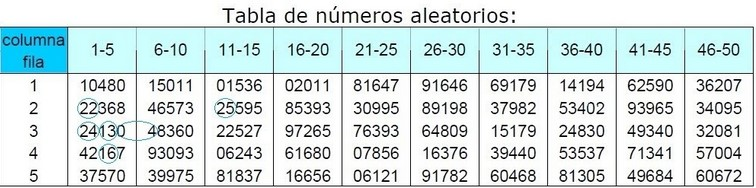
\includegraphics[width=100mm]{includes/ejemplo_tabla.jpg}
 	\caption[Tabla números aleatorios]{Tabla números aleatorios \citep{ejemploReferencia}}
 	\label{ejemploTabla}
 \end{table}
 Como en el caso anterior, la tabla \ref{cochesAfectados} sólo muestra un pequeño porcentaje de coches afectados.
\fi

